\section{Funktionelle krav}\label{sec:funktionelle-krav}

\section{Use Case Diagram}
Nedenunder ses der et use case diagram lavet ud fra medarbejder-mål tabellen. Use case diagrammet giver et godt overblik over, hvilke cases de forskellige aktøre står for, samt kun noget af forholdet mellem aktør, system og use case \cite{visual-paradigm.com}. 

\begin{figure}[H]
    \centering
    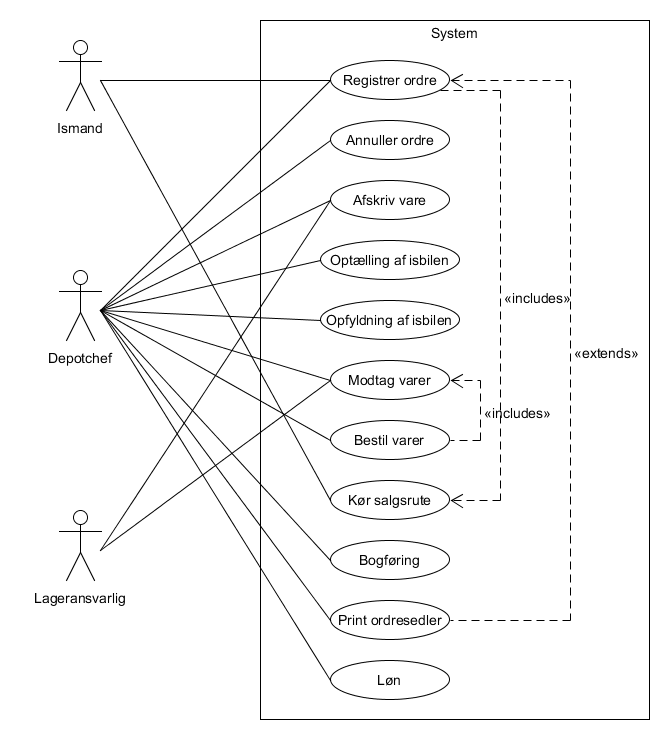
\includegraphics[width=\textwidth]{figures/Forundersøgelse/use_case_diagram.png}
    \caption{Use case diagram}
    \label{fig:use_case_diagram}
\end{figure}

Use Case diagrammet viser at depotchefen står for næsten alle opgaver i virksomheden. Depotchefen udtrykte en interesse for at kunne bruge mindre tid på de mange use cases han har i løbet af dagen, for så at kunne bruge tid på at køre salgsruter. Da det også primært er depotchefen, der står for de opgaver, som udføres i systemet, er det de Use Cases der vil blive fokuseret på.

\section{Fully Dressed}
\begin{longtable}{ |p{120pt}|p{120pt}|p{120pt}| }
    \hline
    Use case navn & Automatisk lagerstyring & \\
    \hline
    Aktør & Depotchefen & \\
    \hline
    Præbetingelser & Et lager med en addresse, penge til at bestille, lagerbeholding fysisk er det samme som i systemet, having a little bit sales data & \\
    \hline
    Postbetingelser & Et lager det er opfylgt med IS & \\
    \hline
    Frekvens & 1 gang om dagen & \\
    \hline
    Main Success Scenario (Flow of events) & Aktørhandling & Systemsvar \\
    \hline
    & 1. vis salgs statistik & 2. en hel masse statistik \\
    \hline
    & 3. klikker "generer lagerplan" & 4. fil dialog omkring hvor planen skal gemmes og er automaitsk sendt til plan-fanen \\
    \hline
    & 5. klikker "load plan" & 6. en eller anden form for UX feedback \\
    \hline
    Alternative flows & 5a. Aktøren vil gerne modificere planen, og gør det i plan-fanen \\
    \hline
\end{longtable}

\begin{longtable}{ |p{120pt}|p{120pt}|p{120pt}| }
    \hline
    Use case navn & Automatisk bogføring & \\
    \hline
    Aktør & Depotchefen & \\
    \hline
    Præbetingelser & ingen & \\
    \hline
    Postbetingelser & bogføring er automatisk færdiggjord i et excel ark & \\
    \hline
    Frekvens & 1 gang om dagen & \\
    \hline
    Main Success Scenario (Flow of events) & Aktørhandling & Systemsvar \\
    \hline
    & 1. klikker "export bogføring" & 2. systemet exporter en excel fil med bogføring \\
    \hline
\end{longtable}